%-----General Settings----%
\documentclass{other/docTemplate}
\svnid{$Id$}

\author{Gonzalo Ducca\formatemail{gonzaloducca@gmail.com} \\ Juan P. Bertone\formatemail{bertonejpb@gmail.com} \\ Juan E. Flórez\formatemail{juan.florez@upr.edu} \\ Valentino Caputa\formatemail{caputavalentino@gmail.com} \\ Carlos Madoery\formatemail{ccmadoery@gmail.com}}  
\po{Melina Griffo\formatemail{Email 1}}
\title{Final Project Report: Life Expectancy} 
\henrymentor{Pía Ruiz}

\loadglsentries{other/acronyms}
\makeglossaries

%-----Beginning of Document----%
\begin{document} 
\maketitle

%---Revision Tracker---%
\startTable
\AddRevision{0.0}{10-20-23}{Document Creation}
\AddRevision{1.0}{11-01-23}{Documentation for Sprint 1}
\stopTable

%-----Table of Contents-----%
\tableofcontents
\listoftables
\listoffigures
\printglossary[title=List of Acronyms ,type=\acronymtype]
\clearpage

%-----Acknowledgments-----%
\section*{Acknowledgments}
\addcontentsline{toc}{section}{Acknowledgments}%adds acknowledgements section to the table of contents

Here is a sample for how to susse acronyms. "Defining a \gls{fr} and a \gls{ps} provides a language for system design. This language is an important aspect of \gls{csd}."
\newpage

%-----Abstract-----%
\section*{Abstract}
\addcontentsline{toc}{section}{Abstract}%adds Abstract section to the table of contents
\newpage

%-----Content-----%
%%%%%%  PROBLEM STATEMENT  %%%%%%                                               
\section{Problem Statement}
What is the problem that you are solving and what do you expect the project to accomplish?

%%%%%%  PROBLEM STATEMENT - Literature Survey  %%%%%% 
\subsection{Literature Survey}
Review the Current Literxature regarding your Problem Statement and Project Description. 
What have other people / companies donde with respect to your problem statement and description? Provide at least five references.

%%%%%%   PROBLEM STATEMENT - State Customer-Defined Constraints & Given Requirements %%%%%%  

\subsection{State Customer-Defined Constraints and Given Requirements}
Determine the Constraints and Given Parameters.
A constraint or given parameteasar affects the selection of all or most of the Functional Requirements and Physical Solutions (PSs) / Design Parameters that your design uses. (i.e., weight, cost, size)

%%%%%%  PROBLEM STATEMENT - State Customer Needs(s)%%%%%%  
\subsection{State Customer Need(s)}
Define Customers and Customer Needs. 
Who are the customers and what are their needs? Consider both internal and external customers. 
Internal customers are the users of the product while external customers are within the company(ies) developing, selling, and distributing the product.


%%%%%%  PROBLEM STATEMENT - Define Use Case(s) %%%%%%  
\subsection{Define Use Case(s)}
Develop Use Cases that define the actions or steps taken by an individual to interact with your system.
Who will operate the system and what must they be able to accomplish?
  

%%%%%%  PROBLEM STATEMENT -System Boundary %%%%%%                      
\subsection{System Boundary}
Define the System Boundary with respect to your project. 
The system boundary distinguishes between what you can control and what your system must interface with (i.e., can't control, but assume to be provided).
Poorly defined interfaces are the number one reason for system failure! 
Define the information that is passed across the system boundary for each of the interfaces. See Fig. \ref{System Boundary}. 

\begin{figure}[ht!]
\centering
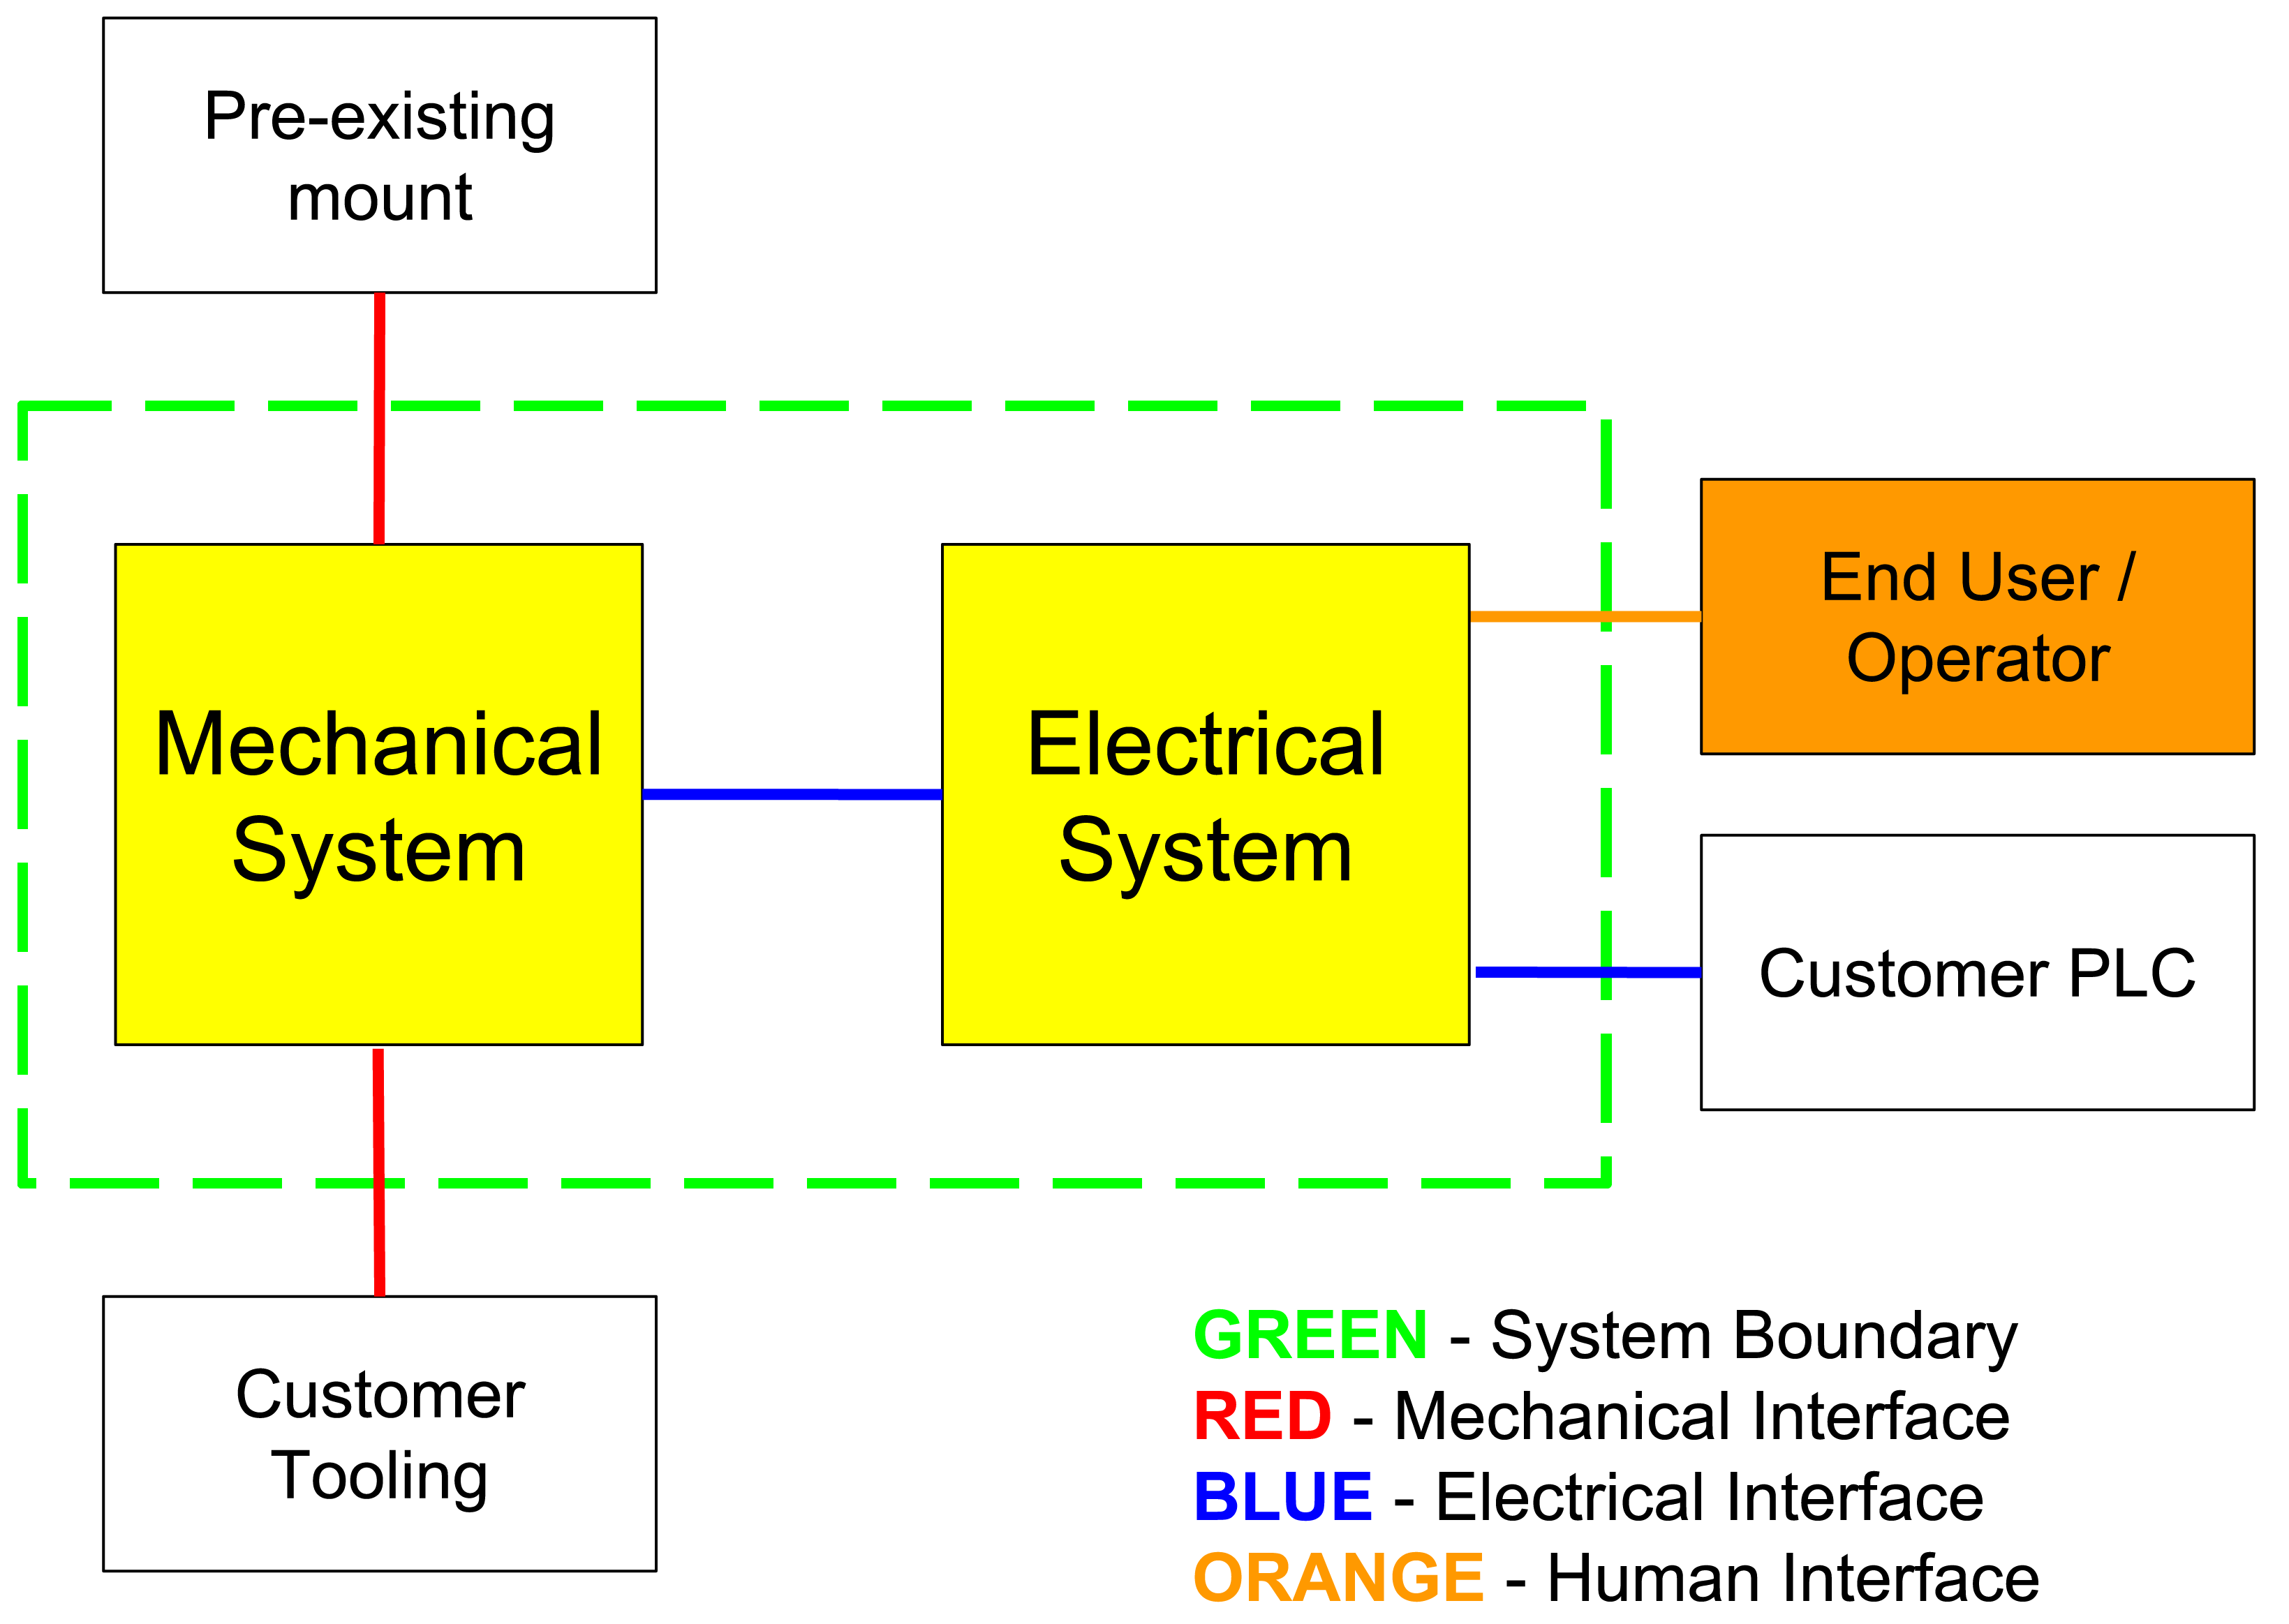
\includegraphics[width=.5\textwidth]{System_Boundary}
\caption{Example of a system boundary diagram}
\label{System Boundary}
\end{figure}



%%%%%%  PROBLEM STATEMENT - Interface Requirements and Definition %%%%%%  

\subsection{Interface Requirements and Definition}

Define the interfaces that exist between items both inside and outside of your system boundary. What information is passed between these entities? 


%%%%%%  Conceptual Design %%%%%%  
\clearpage
\section{Conceptual Designs}
Please provide a brief overview of your conceptual designs. How many conceptual designs do you have, and what makes them different from one another?


%%%%%%   Product Design Map %%%%%%  

\subsection{Product System Design Decomposition}

Translate Customer Needs to your design’s Functional Requirements (FRs). 
A Functional Requirement establishes the design specification (i.e., what the system / product must be able to achieve) based on loosely defined Customer Needs (CNs) - (i.e., "easy to use").  
An FR should have a measurable outcome (FRm).

Develop your high-level (to level 3) design decomposition. 
This is the process of taking high-level FRs and defining detailed PSs in a way that the design is predictable and the sequence and dependencies in hardware/software module implementation is known. 
Your knowledge of the sequence of module implementation is the consequence of applying Design Axiom 1: The Independence Axiom to Maintain Independence of the Functional Requirements.


%%%%%%   Conceptual Design Alternatives %%%%%% 

\subsection{Conceptual Design Alternatives}
Develop Conceptual Design Alternatives (i.e., different Physical Solutions (PSs) / Design Variables / Design Parameters (DPs) to achieve the same FR (i.e., a solution-neutral requirement specification).\\

Conceptual Design Analysis may be based on (can use any combination of these approaches but a minimum of 2 are required):
\begin{itemize}

\item \textbf{Conceptual Design Analysis based on the Product System Design Decomposition}
 For each FR defined, there exists the possibility for alternative solutions (thus the potential for alternative conceptual designs. Based on the physical solution, the lower level functional requirements may vary. The way to represent these solutions with their differing branches is shown in Fig. \ref{Alternatives_Tree}.
%-----------Figure------------%
%\begin{figure}[ht!]
%\centering
%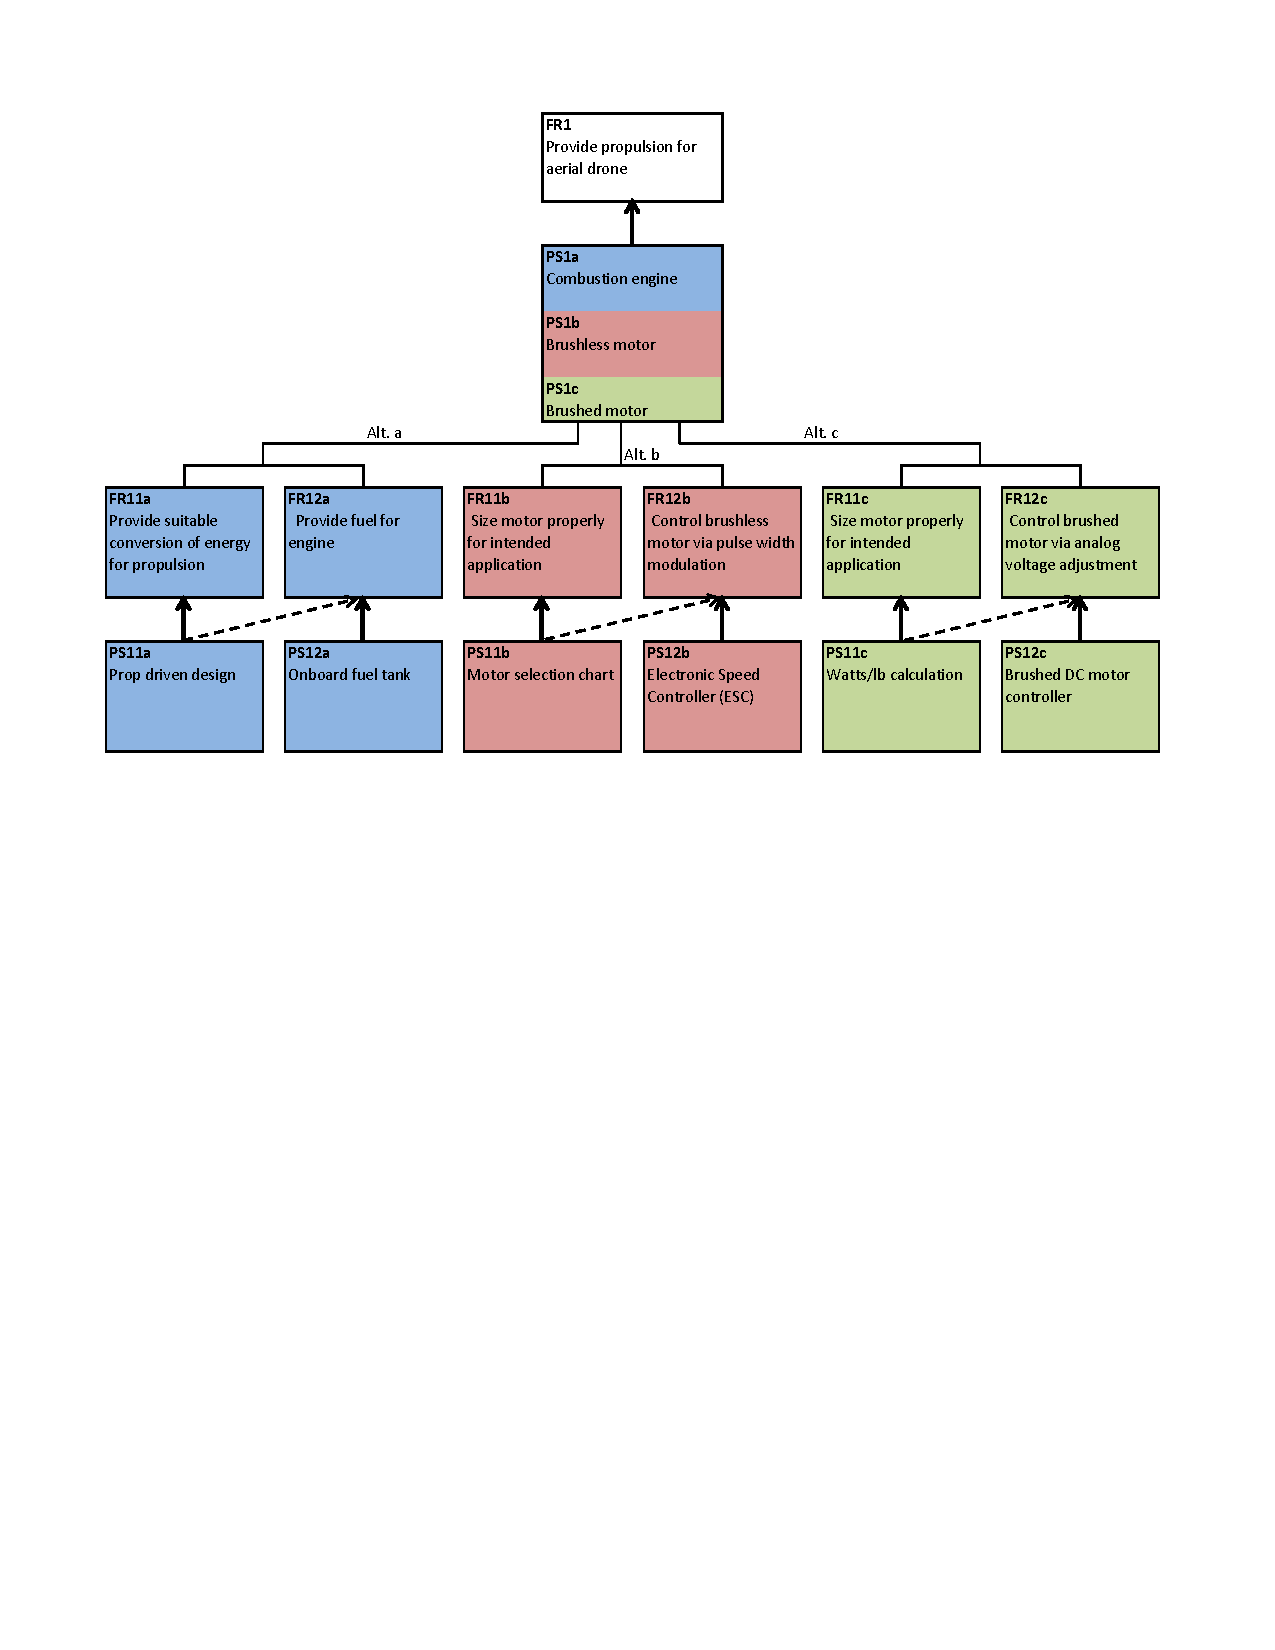
\includegraphics[width=.99\textwidth,]{alternative_tree.pdf}
%\caption{Conceptual Design Alternatives}
%\label{Alternatives_Tree}
%\end{figure}
%-------End of Figure---------%

  \item \textbf{Pugh Concept Selection Matrix} Use the FRs from decomposition as the evaluation criteria. This method is good for a broad assessment of the design alternatives. The drawback can be that the weighting criteria is subjective and results can often be biased.
 

\item \textbf{Process Capability -} the drawback is that it requires time to build a detailed model (i.e.,  Computational Fluid Dynamics (CFD), Finite Element Analysis (FEA), solid model, etc.) and/or physical test to verify whether alternative PS1a, PS1b...  PS1n is the best solution to FR1.\footnote{Suh, Nam P. Complexity: Theory and Applications. Oxford: Oxford UP, 2005. Print.}   A capable process is the Consequence of applying Design Axiom 2: The Information Axiom to Minimize the Information Content (i.e., select design with the highest probability of success).

\end{itemize}

\clearpage
%%%%%%   Evaluation of Design Alternatives %%%%%%  
\section{Evaluation of Design Alternatives}

Please provide an overview for how the conceptual designs were evaluated. How was the criteria chosen? What methods were used to select the best design?

%%%%%%   Criteria for Selection and Testing  %%%%%%  
\subsection{Criteria for Selection and Testing Among Alternatives}

What criteria are used to evaluate the various conceptual designs? This criteria could include factors such as cost, ease of fabrication, etc...


%%%%%%   Design Alternatives Validation Measures %%%%%%  
\subsection{Design Alternatives Validation Plan}

What are the measures that your customer will use to evaluate your design? Does your design alternatives meet these measures? These measures should be defined in your decomposition. For example, a certain tolerance or strength may be required by the customer. In addition, you may determine additional requirements that are key to validating your design. 


%%%%%%   Detailed Design %%%%%%  

\clearpage
\section{Detailed Design}
This section should include the following:full and complete analysis, all calculations, and evaluation. All figures must be computer generated. 

%%%%%%   Design Description and Drawings %%%%%% 
\subsection{Design Description and Drawings}
Provide a detailed description of the chosen conceptual design. This section should include the necessary computer generated drawings to understand your design (i.e CAD drawings, circuit diagrams, etc...)

%%%%%%   Analysis and Calculations %%%%%% 
\subsection{Analysis and Calculations}
Provide the necessary analysis and calculations to detail how the design functions. This analysis should include both the mechanical and electrical calculations if applicable.

%%%%%%   Evaluation %%%%%% 
\subsection{Evaluation}
Provide a summary of the design evaluation. Why are you confident the design will meet the customer's requirements? State the key design equations that you will use to evaluate your design. 


%%%%%% Cost %%%%%% 
\clearpage
\section{Cost}
Provide an overview of the budget provided to you by your industry sponsor. 

%%%%%%  Bill of Materials %%%%%% 

\subsection{Bill of Materials}
Define the Bill of Materials (primary emphasis here is to know what parts must go into your design).


%%%%%%   Cost Estimate %%%%%%  

\subsection{Cost Estimate}
Based on the Bill of Materials, estimate the total cost to build your design. Relate this estimate to the sponsor provided budget.


%%%%%%  Test Development and Execution  %%%%%%  
\clearpage
\section{Risk Mitigation, Design FMEA, and Test Plan}
Provide an overview of why risk assessments are necessary. Explain what tools you used to understand and mitigate the risks associated with your design.
%%%%%%   Risk Mitigation %%%%%%  

\subsection{Risk Mitigation}
Develop a Risk Management Plan to help understand the potential risks along with a corresponding mitigation plan.


%%%%%%  Design FMEA %%%%%%  
\subsection{Design FMEA}
Provide a failure modes and effects analysis for your design. The analysis will show the different ways in which your design could fail (failure modes), and the corresponding severity and likelihood of each risk. 

%%%%%%  Test Plan  %%%%%%  
\subsection{Test Plan for Selected Design Alternative}
Explain why developing a test plan is an important step to product design? 



%%%%%%  Verification Testing %%%%%%  
\subsubsection{Verification Tests}
Provide a test plan for verifying your design.
This test plan should include the required measurements and the units of measure.

%%%%%%  Validation Testing  %%%%%%  
\subsubsection{Validation Tests}
Provide a test plan for validating your design.
This test plan should include the required measurements and the units of measure.

%%%%%%  Test Apparatus%%%%%%  
\subsubsection{Test Apparatus for Each Test}
What equipment/setup is required to complete the various tests defined above? 


%%%%%%  Test Schedule  %%%%%%  
\subsection{Test Schedule}
Define when each test will be completed and in what order.


%%%%%%  Test Results  %%%%%%  
\subsection{Test Results (Second Semester)}
In the second semester, the above test plans will be completed according to your test schedule. The results should be included in your final report for next semester. This section can be commented out for semester one. 
\subsubsection{Verification Results}
What were the results of completing your verification test plan?

\subsubsection{Validation Results}
What were the results of completing your validation test plan?



%%%%%%   Project Timeline  %%%%%%  
\clearpage
\section{Project Plan and Timeline}
\begin{itemize}
\item Develop your design and development schedule that includes both semesters. 
\item Define all activities leading up to key Milestones and Milestone Presentations.
\item Define the date you wisll order materials prior to the conclusion of semester 1. 
Include in your report’s appendix the receipts from ordering material (reference the BOM). 
\end{itemize}

        
%%%%%%   Conclusions  %%%%%%  
\clearpage
\section*{Conclusions and Lessons Learned}
\addcontentsline{toc}{section}{Conclusions and Lessons Learned}%adds Conclusions and Lessons Learned section to the table of contents

Reflect on the dejibassign \cite{gelman2013bayesian} process and your final design \cite{lindquist2008statistical}. What lessons did you learn throughout the process? If you had to redo the whole process, is there anything you would do differently? 


%----References-----%
\clearpage
%Please refer to the OverLeaf Primer to see your options for how to keep track of references.
%\section*{References}
\addcontentsline{toc}{section}{References}%adds reference section to the table of contents
%Use the OverLeaf Primer to understand the different ways to format the references. 
\bibliographystyle{IEEEtran} %Formats the bibliography to meet the IEEE standards
\bibliography{ref.bib} %This command calls a file named "your_references.bib". You will upload this file, and can rename as necessary. 
  

\clearpage
\appendix
 \renewcommand{\thesection}{\Alph{section}.}
\setcounter{section}{0}

\addcontentsline{toc}{section}{Appendices}
%--Product System Design Decomposition----% 
\section{Product System Design Decomposition}
Provide a complete design decomposition. If the different branches relate to different parts of the product design (i.e safety, electrical subsystem, mechanical subsystem, etc...), please label those to show at a high level an overview of your decomposition. 

%Uncomment and use the below commands to include your decomposition. The "angle=90" rotates the decomposition to a landscape view. 

%-----------Figure------------%
% \begin{figure}[ht!]
% \centering
% \includegraphics[width=1.1\textwidth, angle=90]{Design_Decomposition}
% \caption{System Design Map}
% \label{System Design Map}
% \end{figure}
%-------End of Figure---------%


%--Design Drawings/Schematics----% 
\clearpage
\section{Design Drawings/Schematics}
Please provide necessary drawings and schematics here. These should include both the mechanical and electrical figures if applicable. 


%----Appendix Proof of Material Purchase---% 
\clearpage
\section{Proof of Material Purchases}
Please provide a copy of your receipt(s) for the purchase of the items on your bill of materials. 

%----Appendix: Other---% 
\clearpage
\section{Other}

\end{document}
